\section{Model/Implementation Details}\label{sec:Model-Implem-Details}

\subsection{Programming Language}

This is programmed in C++, as the C family of languages are what I am familiar with, and speed is the name of the game here, due to the immense number of calls to complex mathematical routines.

\subsection{Other Tools and Frameworks}

There are two main dependencies that are used, and those are \href{http://gnuplot.info/}{Gnuplot} and \href{https://www.lhapdf.org/}{LHAPDF}. Gnuplot is a simple command-line tool used for plotting data, and it will allow me to visualize results very easily and nicely, and have them be comparable to results from other frameworks. \textsc{LHAPDF} is a package used to interface with \textit{parton distribution functions} (PDFs). These are used to describe the structure of the proton, specifically the probability of finding different quarks within the proton given some momentum fraction $x$. This has to be done this way, by which I mean interfacing with some external package, because the PDFs are not able to be calculated on their own; they have to be determined from experiment and encoded in data file. This is required in the calculational side of things. There is one caveat with this library, and it is that it cannot be built/used on Windows.


\subsection{Structure and Diagrams}

\begin{figure}[ht]
  \centering
  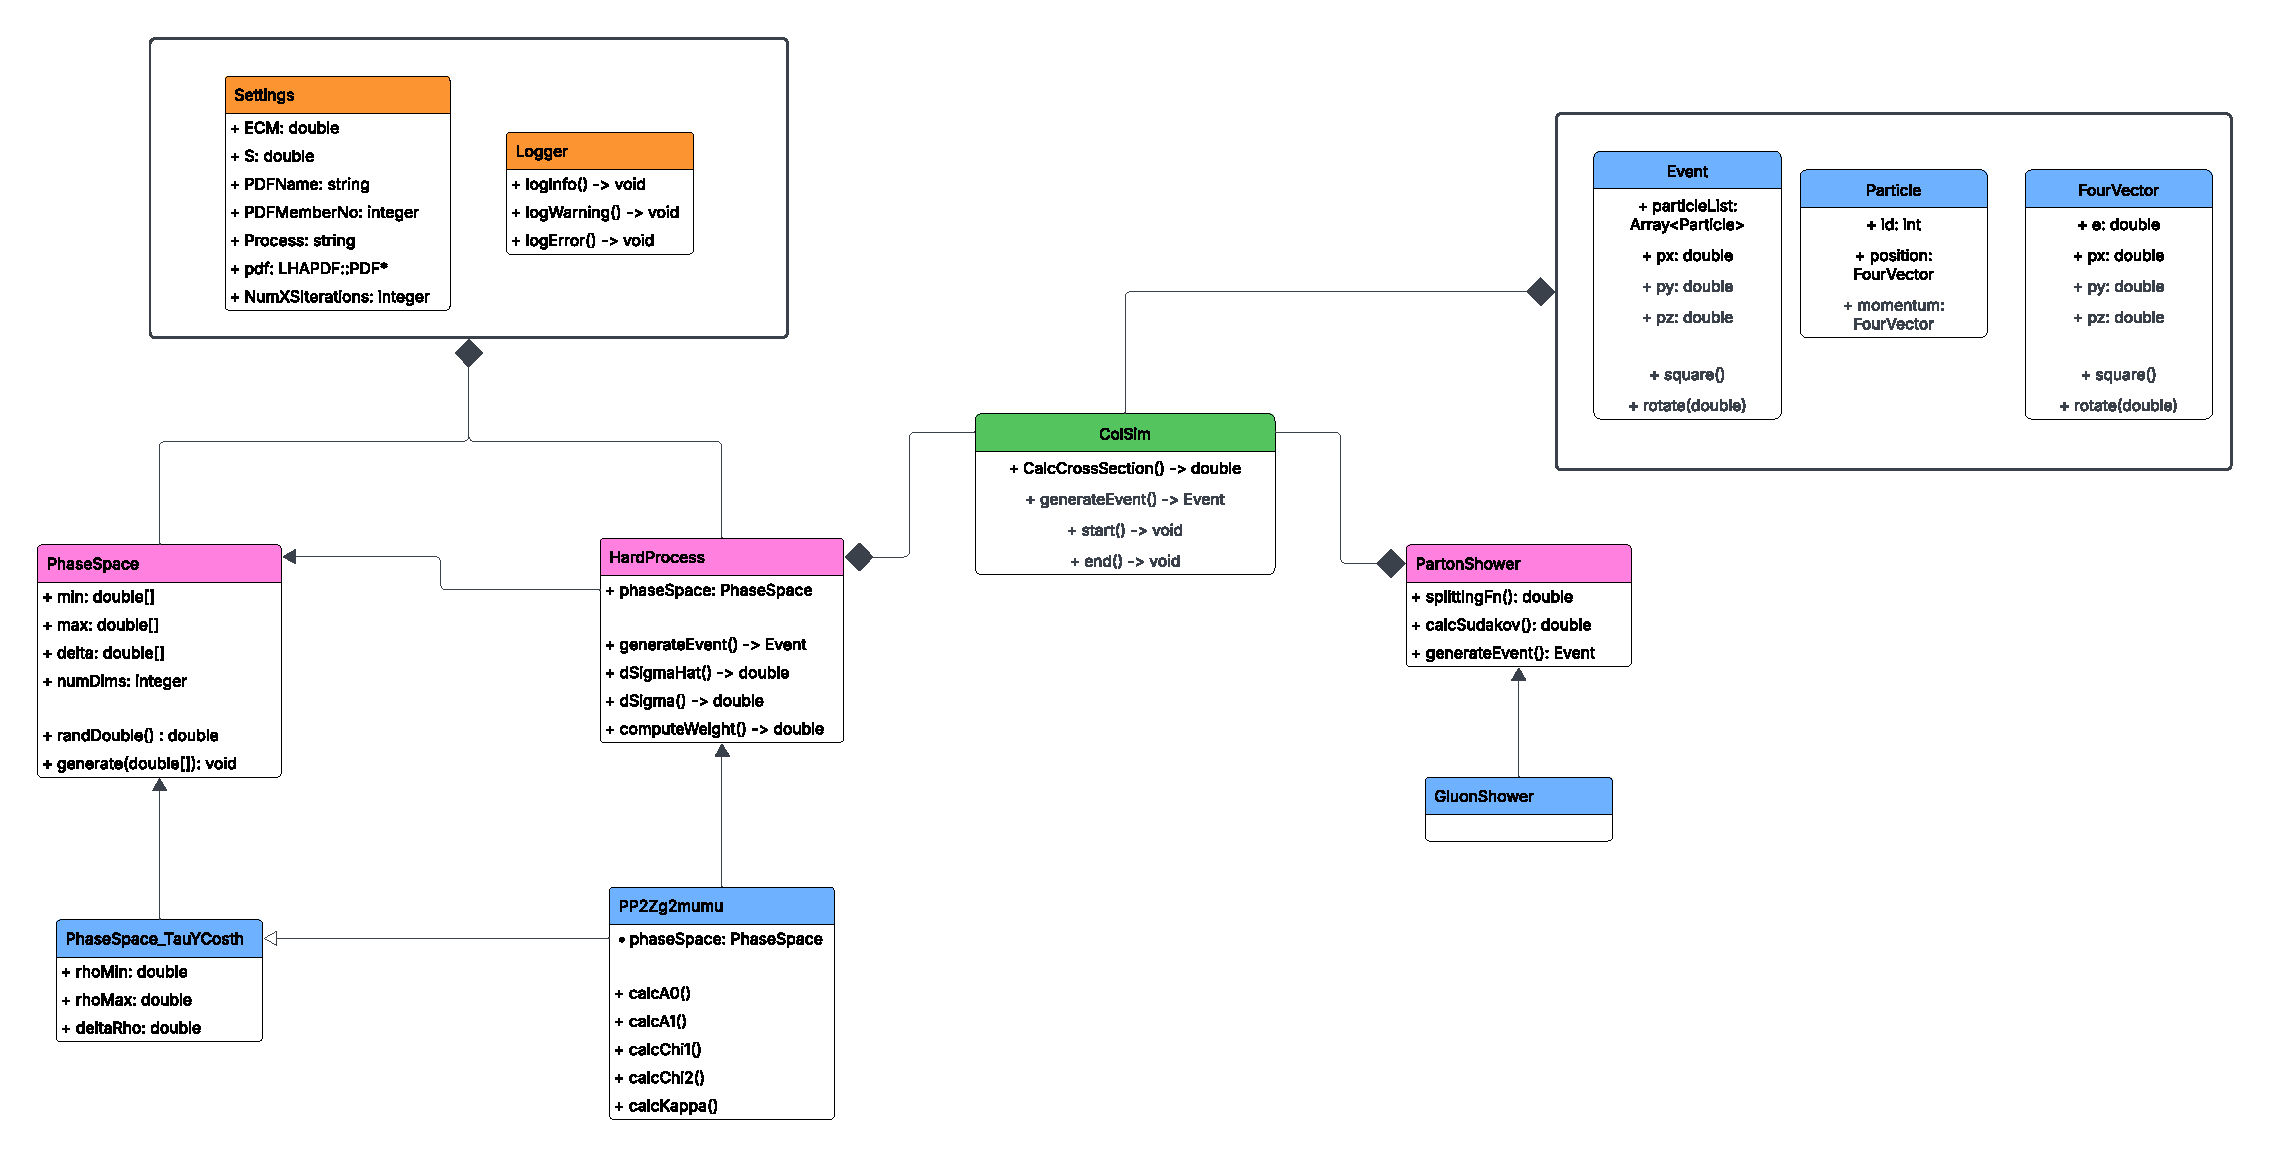
\includegraphics[width=0.9\linewidth]{./res/Images/ColSim_Updated.pdf}
  \caption{Basic UML diagram describing the interaction/relationships between the different classes.}
  \label{fig:uml}
\end{figure}


Given in Fig.~\ref{fig:uml} is the current status of the program in terms of the interactions/relationships between the different classes expressed as a UML diagram.

First, the blocks listed in orange are singleton classes containing functionality that should be available throughout the program via a single interface. The \mintinline{cpp}{Logger} is a class designed at nicely formatting output to a log file and/or standard output/error. In particular, output is given a prefix stating the severity/priority of the message, since some messages are simply messages whereas some are warnings or errors, as well as a time it was outputted, and if your terminal supports it, colors codes.

The \mintinline{cpp}{Settings} class contains things related to reading in data from the configuration file, parsing it, and making it available throughout the program.

The blue blocks are separate classes with no dependencies themselves as they are simple organization of numbers. In particular, this is where data related to particles such as ID, momentum, and so on are stored as well as groups of particles, weight information, and so on. These are referenced throughout the program.

The pink blocks are base classes representing generic behavior for that type of object. The \mintinline{cpp}{PartonShower} class defines common behavior such as the implementation of the Sudakov form factor which should be common for all types of parton showering such as gluon or photon showering. Photon showering, however, turns out to be moderately challenging, so it will not be implemented for this project, but at some point later on it will be, so the general structure remains. Similarly, the \mintinline{cpp}{HardProcess} and \mintinline{cpp}{PhaseSpace} classes contain shared information for all hard process and all of their phase spaces. Just as with the photon showering, additional processes were challenging to implement during this project, so only the single $pp \rightarrow Z/\gamma^* \rightarrow \ell^+\ell^-$ process as been implemented.

Lastly, the single green block is the main entry point for the end user, containing simple methods to initialize the program, generate events, and view output.



\subsection{Current Challenges}

At the moment, the demands of the assignments are indicating an extremely poor choice of project. It is immensely challenging to organize all of the complicated physics involved with even a single process along with the rest of the required components for data retrieval, all while keeping a clean user interface. As such, user control is limited due to the limited implementation of parts of the model, meaning that there is very little to \textit{do} as the user and very little to see. Further, results are not directly comparable yet to other simulation tools out there because of how barebones this is despite the amount of code, physics, and math put into it so far. This is making it harder and harder to put together reports and complete assignments.

Had I the opportunity to choose a different project, I would absolutely have taken it, but I have evidently made this realization far too late. I can only hope that you are generous with your grading and recognize the work I put into this project despite not having results that are as pretty compared to how some of the other students' results are.



%%% Local Variables:
%%% mode: LaTeX
%%% TeX-master: "../../Report"
%%% End:
